%%%%%%%%%%%%%%%%%%%%%%%%%%%%%%%%%%%%%%%%%%%%%%%%%%%%%%%%%%%%%%%%%%%%%%%%%%%%%%%

\chapter{BUSCANDO MAIORES \textit{SPEEDUPS}}
\label{chp:2}

A Tabela \ref{tab:2_flags} detalha as flags de compilação utilizadas para gerar os resultados das Seções \ref{chp:1} e \ref{chp:2}. A Figura \ref{fig:2_hist} ilustra os resultados das execuções com as novas flags. Os novos \textit{Speedups} médios calculados estão na Tabela \ref{tab:2_spedups}; os novos tempos totais estão na Tabela \ref{tab:2_tempos}; a Tabela \ref{tab:2_nloops} indica o número de loops vetorizados e não-vetorizados por cada compilador, com a informação de quantos loops a mais ou a menos foram vetorizados. Nas Tabelas \ref{tab:2_spedups} e \ref{tab:2_tempos} está indicada a alteração relativa $\delta$ das quantidades apresentadas com relação aos resultados da Seção \ref{chp:1}, definida por:

\begin{equation}
\delta = \frac{x_{II}-x_{I}}{x_{I}}, 
\end{equation}

sendo $x_{I}$ e $x_{II}$ os valores das quantidades pertinentes às Seções \ref{chp:1} e \ref{chp:2}, respectivamente. Ou seja, os valores de $x_{I}$ são adotados como referência para quantificar a performance das novas otimizações. 

\renewcommand{\arraystretch}{1.3}
\begin{table}[H]
\center
\caption{Flags de compilação utlizadas nas Seções \ref{chp:1} e \ref{chp:2}.} 
\begin{tabular}{@{}l | l c | c@{}}
\toprule
\multicolumn{2}{@{}l@{}}{ } & \multicolumn{2}{@{}c@{}}{Flags}\\
\cmidrule{2-4}
% -------------------------------
\multicolumn{2}{@{}l@{}}{\texttt{ICC}} &  Seção I & Seção II  \\
\hline  
Otimização base & & \multicolumn{2}{@{}c@{}}{\small \texttt{-std=c99 -O3}} \\
\hline
Vetorização & & \small (ativada via \texttt{-O3} da otim. base) & \small \texttt{-xSSE4.2} \\
\hline
Sem vetorização & & \multicolumn{2}{@{}c@{}}{\small \texttt{-no-vec}} \\
\hline
Relatório de vet. & & \multicolumn{2}{@{}c@{}}{\small \texttt{-qopt-report=2 -qopt-report-phase=vec}} \\
\midrule
% -------------------------------
\multicolumn{2}{@{}l@{}}{\texttt{PGI}} &  Seção I & Seção II  \\
\hline
Otimização base & & \small \texttt{-c99 -O3} & \small \texttt{-c99 -O3 -Mcache\_align} \\
\hline
Vetorização & & \small \texttt{-Mvect=sse} & \small \texttt{-Mvect=sse -Mvect=prefetch} \\
\hline
Sem vetorização & & \multicolumn{2}{@{}c@{}}{\small \texttt{-Mnovect}} \\
\hline
Relatório de vet. & & \multicolumn{2}{@{}c@{}}{\small \texttt{-Minfo}} \\
\midrule
% -------------------------------
\multicolumn{2}{@{}l@{}}{\texttt{GCC}} &  Seção I & Seção II  \\
\hline
Otimização base & & \small \texttt{-O3} & \small \texttt{-O3 -ffast-math} \\
\hline
Vetorização & & \multicolumn{2}{@{}c@{}}{\small \texttt{-ftree-vectorize}} \\
\hline
Sem vetorização & & \multicolumn{2}{@{}c@{}}{\small \texttt{-fno-tree-vectorize}} \\
\hline
Relatório de vet. & & \multicolumn{2}{@{}c@{}}{\small \texttt{-fdump-tree-vect-blocks=report.dump}} \\
\bottomrule
\end{tabular}
\label{tab:2_flags}
\end{table}


\begin{figure}[ht!]
	\vspace{0mm}	% acrescentar o espaçamento vertical apropriado entre o título e a borda superior da figura
	\begin{center}
		\resizebox{\textwidth}{!}{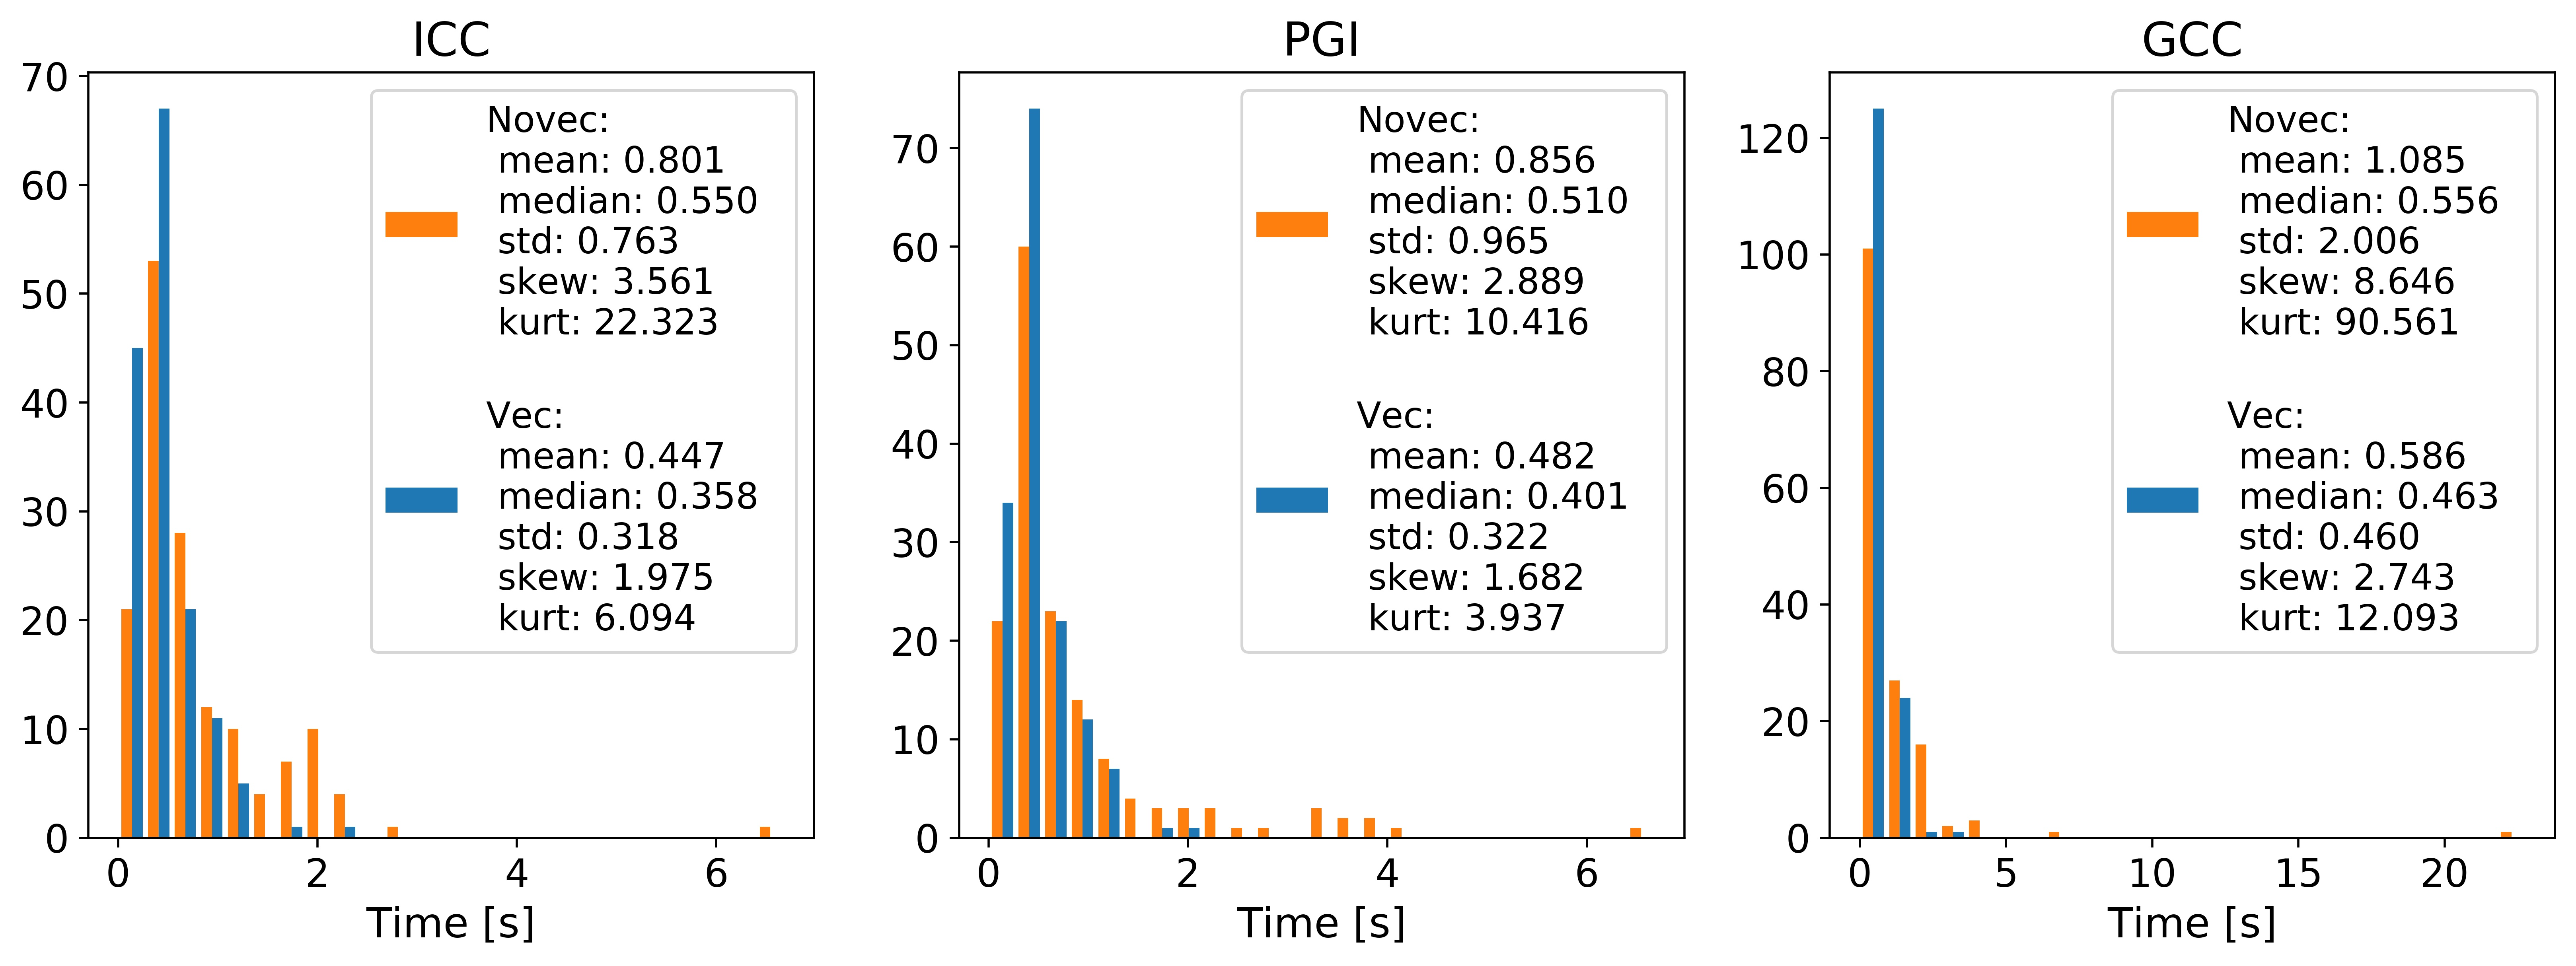
\includegraphics{Figuras/stats2.jpg}}		
	\end{center}
	\vspace{2mm}	% acrescentar o espaçamento vertical apropriado entre a borda inferior da figura e a legenda ou a fonte quando não há legenda (o valor pode ser negativo para subir)
	\caption{Histogramas e estatísticas dos resultados obtidos com as novas flags de compilação. O número de bins é igual a 25.}
	\legenda{}	% legenda - para deixar sem legenda usar comando \legenda{} (nunca deve-se comentar o comando \legenda)
	\label{fig:2_hist}
%	\FONTE{FOnte da imagem (se necessário).}	% fonte consultada (elemento obrigatório, mesmo que seja produção do próprio autor)
\vspace{-8mm}
\end{figure}


\begin{table}[H]
\center
\caption{\textit{Speedups} médios após as novas flags de compilação e seus  $\delta$'s.} 
\begin{tabular}{@{}l l l l@{}}
\toprule
& \texttt{ICC} & \texttt{PGI} &  \texttt{GCC} \\
\midrule
\textit{Speedup} médio & 1.83 & 2.00 & 1.971 \\ 
Alteração relativa ($\delta$) & $+1.1\%$ & $+2.1\%$ & $+39.7\%$ \\ 
\bottomrule
\end{tabular}
\label{tab:2_spedups}
\vspace{-10mm}
\end{table}


\begin{table}[H]
\center
\caption{Tempos totais com as novas flags de compilação seus $\delta$'s.} 
\vspace{-4mm}
\begin{tabular}{@{}l l l l l l l l l@{}}
\toprule
& \multicolumn{2}{@{}c@{}}{\texttt{ICC}} & & \multicolumn{2}{@{}c@{}}{\texttt{PGI}} & &  \multicolumn{2}{@{}c@{}}{\texttt{GCC}} \\
\cmidrule{2-3} \cmidrule{5-6} \cmidrule{8-9}
& Não-vet. & Vet.  & &  Não-vet. & Vet.  & &  Não-vet. & Vet. \\
\midrule
Tempo total [s] & 120.891 &  67.476 & & 129.241 &  72.834 & &  163.855  &  88.499  \\
Alteração relativa ($\delta$) & $0\%$ &  $-0.6\%$ & & $+1\%$ &  $-1.2\%$ & &  $-1.9\%$ & $-34.7\%$ \\
\bottomrule
\end{tabular}
\label{tab:2_tempos}
\vspace{-10mm}
\end{table}


\begin{table}[H]
\center
\caption{Número de loops vetorizados e não-vetorizados (diferença com relação ao resultado anterior entre parênteses).}
\begin{tabular}{@{}l l l l l l l l@{}}
\toprule
\multicolumn{2}{@{}c@{}}{\texttt{ICC}} & & \multicolumn{2}{@{}c@{}}{\texttt{PGI}} & &  \multicolumn{2}{@{}c@{}}{\texttt{GCC}} \\
\cmidrule{1-2} \cmidrule{4-5} \cmidrule{7-8}
Não-vet. & Vet.  & &  Não-vet. & Vet.  & &  Não-vet. & Vet. \\
\midrule
53    &    98 (+4)   &&     99     &    52  (+2)   &&     92   & 59 (+16) \\
\bottomrule
\end{tabular}
\label{tab:2_nloops}
\end{table}
%\begin{figure}[ht!]
%	\caption{Caption: figure example.}
%	\vspace{0mm}	% acrescentar o espaçamento vertical apropriado entre o título e a borda superior da figura
%	\begin{center}
%		\resizebox{13cm}{!}{\includegraphics{Figuras/jpg_omni2_daily_wSxReptBqw.jpg}}		
%	\end{center}
%	\vspace{-2mm}	% acrescentar o espaçamento vertical apropriado entre a borda inferior da figura e a legenda ou a fonte quando não há legenda (o valor pode ser negativo para subir)
%	\legenda{Legend.}	% legenda - para deixar sem legenda usar comando \legenda{} (nunca deve-se comentar o comando \legenda)
%	\label{figfiltrotS0681200}
%	\FONTE{FOnte da imagem (se necessário).}	% fonte consultada (elemento obrigatório, mesmo que seja produção do próprio autor)
%\end{figure}

